We limit now the discussion to the Hartree-Fock basis  we discussed above.
To fourth order in perturbation theory we can produce diagrams with $1p-1h$ intermediate excitations as shown in Fig.~??, $2p-2h$ excitations, see Fig.~??, $3p-3h$ excitations as shown in Fig.~?? and finally so-called diagrams with intermediate four-particle-four-hole excitations, see Fig.~??\footnote{We were unable to render the \texttt{.ps} files.}.

Based on the linked diagram theorem and the form of the pairing Hamiltonian, which diagrams will contribute to fourth order?
Here we recommend reading Shavitt and Bartlett's chapter 4--6, and chapter 6 in particular about the linked diagram theorem.

Calculate the energy to fourth order with the Hartree-Fock basis defined earlier for $g \in [-1,1]$ and compare with the full diagonalization case in exercise 2). % chktex 10 % tex-fmt: skip
Discuss the results.

\subsection{}
Based on the pairing nature of the Hamiltonian, we can immediately exclude the $1p-1h$ and $3p-3h$ diagrams.
We can furthermore reduce the possible $2p-2h$ diagrams to diagrams 5, 6, 14, 15.
The $4p-4h$ diagrams which are possible based on the pairing, are diagrams 33, 36, 37 and 41.

With diagrams 33 and 41, we now have to be careful as they are unlinked diagrams.
By the linked diagram theorem, we can exlude these diagrams, and only consider the contributions from the linked diagrams, rather than considering the principal and renormalization terms.

Beginning with diagrams 5 and 6, both have $n_h = 4$, $n_l = 2$ and $n_{ep} = 4$.
As the notation is quite wieldy, we adopt the convention of writing
\begin{equation*}
    \varepsilon_i^a = \varepsilon_i - \varepsilon_a, \quad \varepsilon_{ij}^{ab} = \varepsilon_i + \varepsilon_j - \varepsilon_a - \varepsilon_b, \quad \text{etc.}
\end{equation*}
The contributions from these diagrams are then
\begin{align*}
    (5) \quad& (-1)^6 \frac{1}{2^4} \sum_{\substack{abcd \\ ijkl}} \frac{
        \langle ij \vert V \vert kl \rangle
        \langle kl \vert V \vert cd \rangle
        \langle cd \vert V \vert ab \rangle
        \langle ab \vert V \vert ij \rangle
    }{
        \varepsilon_{ij}^{ab} \cdot
        \varepsilon_{kl}^{ab} \cdot
        \varepsilon_{kl}^{cd}
    } \\
    (6) \quad& (-1)^6 \frac{1}{2^4} \sum_{\substack{abcd \\ ijkl}} \frac{
        \langle ij \vert V \vert kl \rangle
        \langle kl \vert V \vert cd \rangle
        \langle cd \vert V \vert ab \rangle
        \langle ab \vert V \vert ij \rangle
    }{
        \varepsilon_{ij}^{ab} \cdot
        \varepsilon_{ij}^{cd} \cdot
        \varepsilon_{kl}^{cd}
    }
\end{align*}
which by the previous method simplify to
\begin{align*}
    (5) \quad& \frac{1}{128} \sum_{\substack{ac\\ik}} \frac{
        g^4
    }{
        (i - a)(k - a)(k - c)
    } \\
    (6) \quad& \frac{1}{128} \sum_{\substack{ac\\ik}} \frac{
        g^4
    }{
        (i - a)(i - c)(k - c)
    }
\end{align*}
summing now just over energy levels.

For diagrams 14 and 15 we have $n_h = 2$ and $n_h = 6$ respectively, with $n_l = 2$ and $n_{ep} = 4$.
The contributions from these diagrams are then
\begin{align*}
    (14) \quad& (-1)^4 \frac{1}{2^4} \sum_{\substack{abcdef \\ ij}} \frac{
        \langle ij \vert V \vert ef \rangle
        \langle ef \vert V \vert cd \rangle
        \langle cd \vert V \vert ab \rangle
        \langle ab \vert V \vert ij \rangle
    }{
        \varepsilon_{ij}^{ab} \cdot
        \varepsilon_{ij}^{cd} \cdot
        \varepsilon_{ij}^{ef}
    } \\
    (15) \quad& (-1)^8 \frac{1}{2^4} \sum_{\substack{ab \\ ijklmn}} \frac{
        \langle ij \vert V \vert kl \rangle
        \langle kl \vert V \vert mn \rangle
        \langle mn \vert V \vert ab \rangle
        \langle ab \vert V \vert ij \rangle
    }{
        \varepsilon_{ij}^{ab} \cdot
        \varepsilon_{kl}^{ab} \cdot
        \varepsilon_{mn}^{ab}
    }
\end{align*}
which simplify to
\begin{align*}
    (14) \quad& \frac{1}{128} \sum_{\substack{ace\\i}} \frac{
        g^4
    }{
        (i - a)(i - c)(i - e)
    } \\
    (15) \quad& \frac{1}{128} \sum_{\substack{a\\ikm}} \frac{
        g^4
    }{
        (i - a)(k - a)(m - a)
    }
\end{align*}

For diagram 36 we have $n_h = 4$, $n_l = 0$ and $n_{ep} = 4$, and then the expression
\begin{equation*}
    (36) \quad (-1)^6 \frac{1}{2^4} \sum_{\substack{abcd \\ ijkl}} \frac{
        \langle ij \vert V \vert cd \rangle
        \langle cd \vert V \vert kl \rangle
        \langle kl \vert V \vert ab \rangle
        \langle ab \vert V \vert ij \rangle
    }{
        \varepsilon_{ij}^{ab} \cdot
        \varepsilon_{ijkl}^{abcd} \cdot
        \varepsilon_{ij}^{cd}
    }
\end{equation*}
which simplifies to
\begin{equation*}
    (36) \quad \frac{1}{128} \sum_{\substack{ac\\ik}} \frac{
        g^4
    }{
        (i - a)(i + k - a - c)(i - c)
    }.
\end{equation*}
By symmetry, we have
\begin{equation*}
    (37) \quad \frac{1}{128} \sum_{\substack{ac\\ik}} \frac{
        g^4
    }{
        (i - a)(i + k - a - c)(k - a)
    }.
\end{equation*}

Performing the summations, we get an additional contribution to the energy of
\begin{equation*}
    -\frac{2063}{13824} g^4 \approx -0.149 g^4.
\end{equation*}
For higher and higher powers, the additional contributions become smaller for values of $g$ further from $\pm 1$.
As we see in Figs.~\ref{fig:rs4_energy} and~\ref{fig:rs4_diff}, the fourth-order RSPT seem to be a worse approximation, as compared with the third-order RSPT. % chktex 13
This is not an entirely unexpected result, as pertubation theories give no guarantees of better convergence for each higher term included.
Again, the approximate energy falls below the exact energy computed with FCI, as RSPT is not variational.

\begin{figure}[htbp]
    \centering
    \begin{subfigure}[b]{0.45\textwidth}
        \centering
        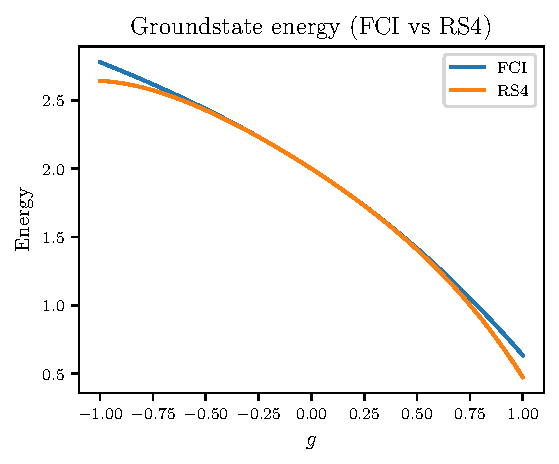
\includegraphics[width=\textwidth]{figures/g_groundstate_energy.pdf}
        \caption{
            Groundstate energy from RSPT.\label{fig:rs4_energy}
        }
    \end{subfigure}
    \hfill
    \begin{subfigure}[b]{0.48\textwidth}
        \centering
        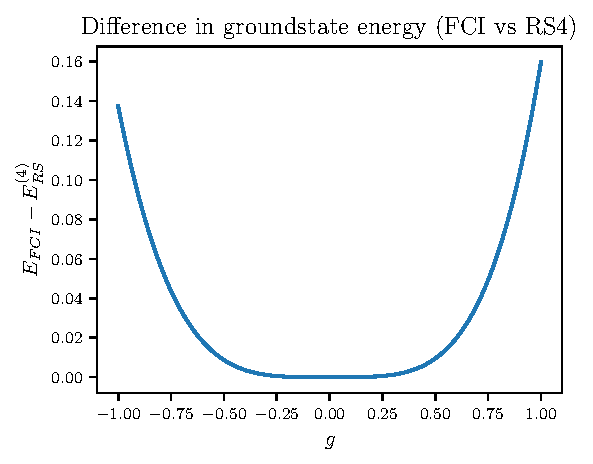
\includegraphics[width=\textwidth]{figures/g_groundstate_energy_diff.pdf}
        \caption{
            Difference in energy from RSPT.\label{fig:rs4_diff}
        }
    \end{subfigure}
    \caption{
        Groundstate energy from the Rayleigh-Schr\"odinger perturbation theory to fourth-order, compared with the FCI results, as a function of $g$.
    }
\end{figure}
